\title{Homework 4 Solutions for Computer Logic and Circuit Design: PHYS306/COSC330}
\author{Dr. Jordan Hanson - Whittier College Dept. of Physics and Astronomy}
\date{\today}
\documentclass[10pt]{article}
\usepackage[a4paper, total={18cm, 27cm}]{geometry}
\usepackage{graphicx}
\usepackage{amsmath}
\begin{document}
\maketitle

\section{6-2,6-3: Parallel Binary Adders, and Ripple-Carry and Look-Ahead Adders}

\begin{enumerate}
\item Exercise 4: Consulting the truth table, we should get $\vec{\Sigma} = (1,1,0,0)$ and $\vec{C}_{out} = (0,1,1)$.  The fourth carry out is the MSB of $\Sigma$.  111+101 = 1100.
\item Exercise 7: Given that the switch line is high, the XNOR gates just pass the original value of $\vec{B}$.  Thus, it turns into an \textit{adder} rather than a \textit{subtracter}.  The output is 10101 (final carry-out is 1, with $\vec{\Sigma} = (0,1,0,1)$.
\item Exercise 11: The book says 40 ns + 6 * 25 ns + 35 ns = 225 ns, for each stage adding all 1's.  I would also accept 8 * 40 ns if you were thinking about the cumulative delay vs. the time between first input and last output.
\end{enumerate}

\section{6-4: Comparators}

\begin{enumerate}
\item Exercise 15: a) $A>B$ true, else false, b) $A<B$ true, else false, c) $A=B$ true, else false
\end{enumerate}

\section{6-5: Decoders}

\begin{enumerate}
\item Exercise 20: See Fig. \ref{fig:exer20}, left.  The key is generating first the SOP and evaluating it by time-steps.
\item Exercise 21: See Fig. \ref{fig:exer20}, right.  The key is decoding each binary number and assigning it to the correct output line.  Remember that these decoders are active LOW.
\begin{figure}[hb]
\centering
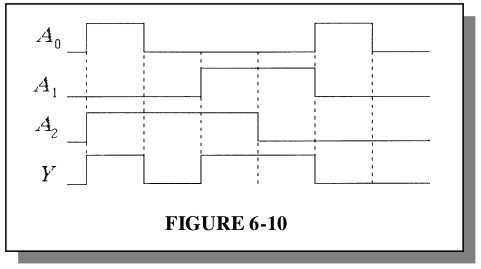
\includegraphics[width=0.35\textwidth]{exercise20.png}
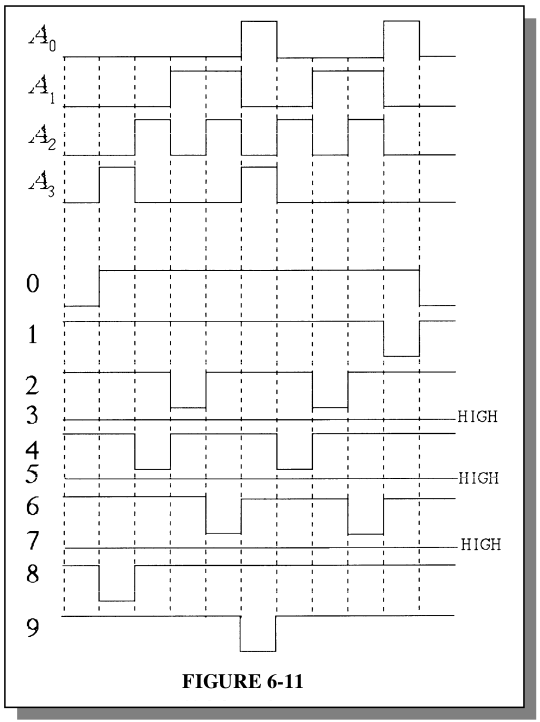
\includegraphics[width=0.35\textwidth]{exercise21.png}
\caption{\label{fig:exer20} Solution to Exercise 20.}
\end{figure}
\end{enumerate}

\section{6-6: Encoders}

\begin{enumerate}
\item Exercise 23: The result is 1011, which is not a valid BCD code.
\end{enumerate}

\section{6-9: Multiplexers}

\begin{enumerate}
\item See Fig. \ref{fig:exer29}).
\begin{figure}[hb]
\centering
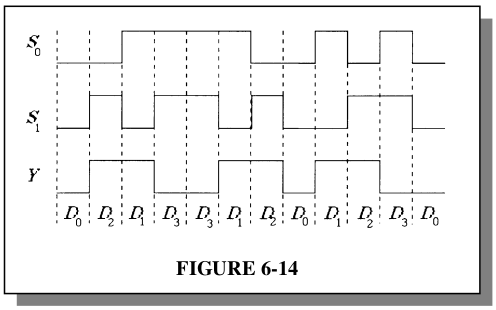
\includegraphics[width=0.35\textwidth]{exercise29.png}
\caption{\label{fig:exer29} Solution to Exercise 29.}
\end{figure}
\end{enumerate}

\section{6-11: Troubleshooting}

\begin{enumerate}
\item In this example, we see right away that the output pins don't correspond to the regular results of an adder.  The results suggest that $C_{in}$ is always HIGH, regardless of the \textit{input} to $C_{in}$.
\end{enumerate}

\section{Special Design Problem}

\begin{enumerate}
\item Exercise 45: The Karnaugh Map for $C_{out}$ yields $BC_{in} + AC_{in} + AB$.  The Karnaugh Map for $\Sigma$ yields $\bar{A}\bar{B}C_{in} + \bar{A}B\bar{C}_{in} + ABC_{in} + A\bar{B}\bar{C}_{in}$.  THe first is a simplification but the second is not.  See Fig. \ref{fig:exer45} for the attachments to 8-to-1 mux inputs that yield these expressions.
\begin{figure}[hb]
\centering
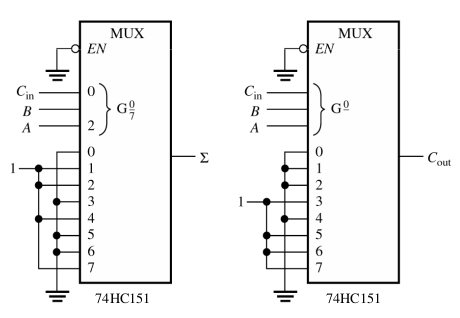
\includegraphics[width=0.5\textwidth]{exercise45.png}
\caption{\label{fig:exer45} Solution to Exercise 45.}
\end{figure}
\end{enumerate}

\end{document}
